\documentclass[tikz]{standalone}
\usetikzlibrary{shapes.geometric}
\begin{document}%
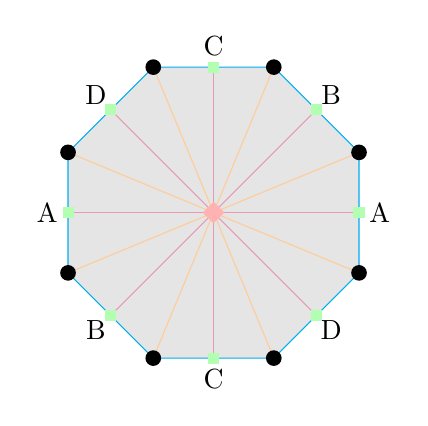
\begin{tikzpicture}[scale=2]
\coordinate (C) at (0,0);

\coordinate (A0) at (45/2:1cm);
\coordinate (A1) at (135/2:1cm);
\coordinate (A2) at (225/2:1cm);
\coordinate (A3) at (315/2:1cm);
\coordinate (A4) at (405/2:1cm);
\coordinate (A5) at (495/2:1cm);
\coordinate (A6) at (585/2:1cm);
\coordinate (A7) at (675/2:1cm);

\coordinate (B0) at (barycentric cs:A7=1,A0=1);
\coordinate (B1) at (barycentric cs:A0=1,A1=1);
\coordinate (B2) at (barycentric cs:A1=1,A2=1);
\coordinate (B3) at (barycentric cs:A2=1,A3=1);
\coordinate (B4) at (barycentric cs:A3=1,A4=1);
\coordinate (B5) at (barycentric cs:A4=1,A5=1);
\coordinate (B6) at (barycentric cs:A5=1,A6=1);
\coordinate (B7) at (barycentric cs:A6=1,A7=1);

\fill[gray!20] (A7) -- (A0) -- (A1) -- (A2) -- (A3) -- (A4) -- (A5) -- (A6) -- (A7);

\node at (barycentric cs:C=-.25,A7=1,A0=1) {A};
\node at (barycentric cs:C=-.25,A0=1,A1=1) {B};
\node at (barycentric cs:C=-.25,A1=1,A2=1) {C};
\node at (barycentric cs:C=-.25,A2=1,A3=1) {D};
\node at (barycentric cs:C=-.25,A3=1,A4=1) {A};
\node at (barycentric cs:C=-.25,A4=1,A5=1) {B};
\node at (barycentric cs:C=-.25,A5=1,A6=1) {C};
\node at (barycentric cs:C=-.25,A6=1,A7=1) {D};


\draw[purple!40] (B0) -- (B4);
\draw[purple!40] (B1) -- (B5);
\draw[purple!40] (B2) -- (B6);
\draw[purple!40] (B3) -- (B7);

\draw[orange!40] (A0) -- (A4);
\draw[orange!40] (A1) -- (A5);
\draw[orange!40] (A2) -- (A6);
\draw[orange!40] (A3) -- (A7);

\draw[cyan] (A7) -- (A0) -- (A1) -- (A2) -- (A3) -- (A4) -- (A5) -- (A6) -- (A7);


\node[diamond,fill=red!30,inner sep=2pt] at (C) {};
\foreach \x in {0,1,...,7}
{
  \node[circle,fill=black,inner sep=2pt] at (A\x) {};
  \node[rectangle,fill=green!30,inner sep=2pt] at (B\x) {};
}
\end{tikzpicture}%
\end{document}
